\documentclass[autodetect-engine,dvipdfmx-if-dvi,ja=standard]{bxjsarticle}

% 二段組にするとき
% \documentclass[twocolumn,autodetect-engine,dvipdfmx-if-dvi,ja=standard]{bxjsarticle}

\usepackage{graphicx}        %図を表示するのに必要
\usepackage{color}           %jpgなどを表示するのに必要
\usepackage{amsmath,amssymb} %数学記号を出すのに必要
\usepackage{setspace}
\usepackage{eclclass}
\usepackage{cases}
\usepackage{here}
\usepackage{fancyhdr}
\usepackage{ascmac}

% 文書全体のスタイルを設定(主に余白)
\setlength{\topmargin}{-0.3in}
\setlength{\oddsidemargin}{0pt}
\setlength{\evensidemargin}{0pt}
\setlength{\textheight}{44\baselineskip}

% 行頭の字下げをしない
\parindent = 0pt

% ヘッダとフッタの設定
\lhead{電気情報工学応用実験II}
\chead{}
\rhead{5E 20番 佐藤凌雅}
\lfoot{}
\cfoot{-\thepage-} % ページ数
\rfoot{}

% 式の番号を(senction_num.num)のようにする
\makeatletter
\@addtoreset{equation}{section}
\def\theequation{\thesection.\arabic{equation}}
\makeatother

% 画像の貼り付けを簡単にする
\newcommand{\pic}[2]
{
  \begin{figure}[H]
    \begin{center}
      \includegraphics[scale=#2]{#1}
    \end{center}
  \end{figure}
}

% 単位の記述を簡単にする
\newcommand{\unit}[1]
{
  \, [\mathrm{#1}]
}
\begin{document}
% \maketitle
\pagestyle{fancy}
\section{目的}
 磁束計を用いて電気機器用鉄板の$B$-$H$曲線を求め,さらにエプスタイン装置を用いて鉄損を測定し,変圧器,直流機ならびに交流機に使用される電気用鉄板の磁気特性の概念を得る.\\

\section{理論}
\subsection{ヒステリシス損}
 鉄の分子相互間の摩擦によって生じる損失のこと.\\
 ヒステリシス損は鉄心内磁束の大きさ,方向の変動により鉄心中の磁気分子の方向,配列が変化し,分子相互間の摩擦損を生ずることによるもので,ヒステリシスループの囲む面積に比例する.\\
 電圧の2乗に比例し周波数に反比例する.鉄損中,約80[\%]はヒステリシス損で,ヒステリシス損は鉄板の厚みには無関係である.
\footnote{ヒステリシス損とは - E\&M JOBS,https://em.ten-navi.com/dictionary/2758/,2019-7-9閲覧}

\subsection{渦電流損}
 導体の一部で磁束が変化したり,磁束が導体を切ったりすると,電磁誘導作用によってその導体内部に起電力を誘起し,その部分だけに電流が流れる.この電流を渦電流という.このように渦電流が流れるとその通路は抵抗をもっているので電力損失を生じ,ジュール熱のために温度が上昇する.この損失を渦電流損という.\\
 変圧器や発電機,電動機などは多量の鉄心を用い,また多くのコイルを巻くため,鉄塊のままでは渦電流損が大きくなる.
\footnote{渦電流損とは - E\&M JOBS,https://em.ten-navi.com/dictionary/2759/,2019-7-9閲覧}

\section{実験回路図}
\begin{figure}[H]
  \centering
  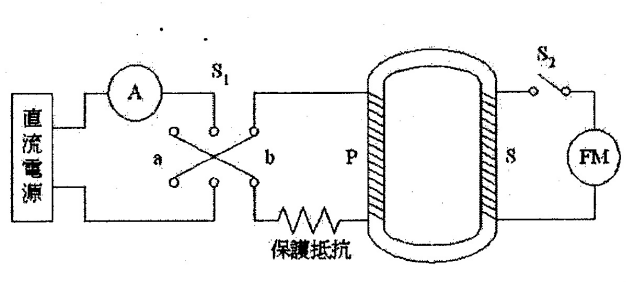
\includegraphics[width=13cm]{./fig/1.png}
  \caption{磁束計による電気機器用鉄板の$B$-$H$曲線の測定}
\end{figure}

\begin{figure}[H]
  \centering
  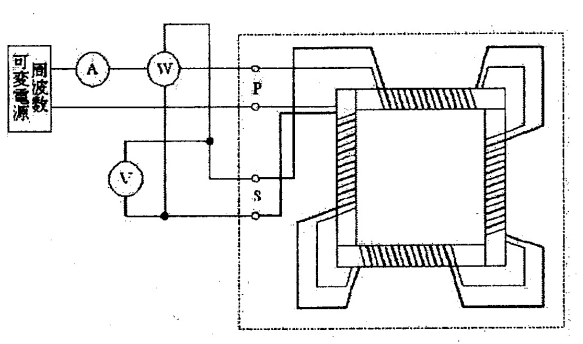
\includegraphics[height=7cm]{./fig/2.png}
  \caption{エプスタイン装置による電気鉄板の鉄損測定}
\end{figure}

\section{実験方法}
\subsection{磁束計による電気機器用鉄板の $B$-$H$ 曲線の測定}
\subsubsection{磁束の測定}
\begin{enumerate}
  \item 図1の通りに結線する.
  \item 試料の減磁作業を行う.磁束計スイッチ S2 を OFF にして,電源電圧を 0 から徐々に上昇させながら,S1を1回/秒ほどの割合で a⇄b側を切り換える.電流値が 1A 程度になったら,徐々に電流値0A まで減少させながら同様に S1を切り換える.
  \item 磁束計スイッチ S2 を「SHORT」にして,S2 を 2,3回程度押してゼロ調整を行う.
  \item 電源電圧を調整して電流値を 0.1A に設定して,S1を OFF から a側に入れて磁束計を読む.
  \item S1 を b側に切り換えて同様に磁束計を読む.この測定を2,3回程度繰り返して平均値を求める.
  \item 電流値を最大 1A まで変化させて測定する.
  \item 測定値から4.1.2を使用して各諸量を計算する.
\end{enumerate}


\subsubsection{諸量の計算}
\begin{enumerate}
  \item 磁束$\phi$の計算
  使用している磁束計 (TFM-2000) で読み $X$ の単位は [mWb] である.また,電気機器用鉄板の二次巻線巻数は 25 である.これらの数値から 式(1) より,鉄板中の磁束 [Wb] を求める.
  \begin{flalign}
    \phi = \frac{X}{25}
  \end{flalign}\\

  \item 磁界 $H$ の計算
  平均磁路の長さ $L$ = 0.32[m],一次巻線の巻数 $N_1$ = 160 である.これらの数値から 式(2) より,磁界の強さ $H$[A/m] を求める.
  \begin{flalign}
    H=\frac{IN_1}{L}
  \end{flalign}\\

  \item 磁束密度 $B$ の計算
  試料の断面は,縦 30mm,横20mm である.これより断面積 $A$[$\mathrm{m^2}$] を求め,式(3) より磁束密度 $B$[T] を求める.
  \begin{flalign}
    B=\frac{\phi}{A}
  \end{flalign}\\

  \item 透磁率 $\mu$ の計算
  式(4) より,透磁率 $\mu$[H/m] を求める.
  \begin{flalign}
    \mu = \frac{B}{H}
  \end{flalign}\\
\end{enumerate}


\subsection{エプスタイン装置による電気鉄板の鉄損測定}
\subsubsection{鉄損計算のための電力ならびに電圧測定}
\begin{enumerate}
  \item 図2の通りに結線する.
  \item 電源周波数を 50Hzに設定し,電源の出力電圧を変えて一次巻線 P の電流を段階的に変化させ,これに対する電力計と電圧計の読みを記録する.
  \item 周波数を60Hzに設定し同様の測定を行う.
  \item 測定値から Sec.4.2.2 を使用して各諸量を計算する.
\end{enumerate}

\subsubsection{諸量の計算}
\begin{enumerate}
  \item 鉄損 $W_i$の計算
  電圧計ならびに電流計の読みと,これらの電圧コイル等の抵抗値から,計器の銅損を除いた単位重量当たりの鉄損 [W/kg] は 式(5) で求めることができる.
  \begin{flalign}
    W_i = \frac{1}{M} \left( W_0 - E_0^2 (\frac{1}{R_V} + \frac{1}{R_W}) \right)
  \end{flalign}
  $E_0$:電圧計の読み [V]\\
  $W_0$:電力計の読み[W]\\
  $R_V$:電圧計の電圧コイルの抵抗値 [$\Omega$]\\
  $R_W$:電力計の電圧コイルの抵抗値 [$\Omega$]\\
  $M$: 重量 [kg]\\

  \item 磁化電流 $I_n$ の計算
  磁化電流 [A] は,電流計の読みからその有効分電流を減じたものであるから 式(6)で求めることができる.
  \begin{flalign}
    I_m = \sqrt{I_0^2 - \left( \frac{W_0}{E_0} \right)^2}
  \end{flalign}
  $\frac{W_0}{E_0}$:有効分電流[A]\\

  \item 磁界 (磁化力)の最大値H/mの計算
  磁界の最大値 [A/m] は,鉄心の平均長さ,磁化電流の大きさならびに磁化コイル巻数より,式(7)で求めることができる.
  \begin{flalign}
    H_m = \frac{1}{L} \left( \sqrt{2} I_m N \right)
  \end{flalign}
  $N$:磁化コイル巻数[回]\\
  $L$:鉄心の平均長さ[m]\\

  \item 最大磁束密度 $B_m$の計算
  誘導起電力と最大磁束密度には比例の関係があり,その与えられる関係式を変形すると,最大磁束密 度は 式(8) で求めることができる.
  \begin{flalign}
    E_0 &= 4.44 f A B_m N \nonumber\\
    B_m &= \frac{E_0}{4.44 f A N}
  \end{flalign}
  $f$:周波数[Hz]\\
  $A$:鉄心の断面積[$m^2$]\\
  $N$:巻数[回]\\

  \item 透磁率$\mu_e$の計算
  最大磁束密度と磁界の最大値より,透磁率$\mu_e$[H/m] は 式(9) で求めることができる.
  \begin{flalign}
    \mu_e = \frac{B_m}{H_m}
  \end{flalign}
\end{enumerate}

\section{使用機器}
\subsection{磁束計による電気機器鉄板の$B$-$H$曲線の測定}
 磁束計:FLUX METER,TFM-200 TOYO MEASURING SYSTEM CO.LTD. ,S/N 7A00669\\
 電流計:YEW AMPERES,1965,NO.52B171\\
 直流電源:REGURATED DC POWER SUPPLY,MODEL PAB 18-3,48245155 AC 100V 50/60Hz\\
 切り替えスイッチ:30A,250V,41-9346 MDM\\

\subsection{エプスタイン装置による電気鉄板の鉄損測定}
 エプスタイン装置:25cm EPSTEIN CORE LOSS TESTER,TYPE B-EP-25 5038B20 1965,\\  YOKOGAWA ELECTRIC WORKS.LTD\\
 電力計:YEW WATTS SNGLE-PHASE 1965 NO.5147C225\\
 低周波定電圧電源:CVFT1-200H,東京精電株式会社 VVVF POWER SUPPY,SER-NO TC-06449\\
 電流計:Sanwa CD800A 15025013602\\
 電圧計:Sanwa CD800A 15025013608\\


% \newpage
\section{実験結果}
\subsection{磁束計による電気機器用鉄板の $B$-$H$ 曲線の測定}
 実験結果を表1,表2及び図3に示す.\\

\subsection{エプスタイン装置による電気鉄板の鉄損測定}
 実験結果を表2から表4,及び図4から図6に示す.

\begin{landscape}
  \begin{table}[p]
    \centering
    \small
    \caption{磁束の測定}
    \scalebox{0.61} {
      \begin{tabular}{rrr}
\toprule
\multicolumn{1}{c}{照度(目標値)[lx]} & \multicolumn{1}{c}{照度(実測値)[lx]} & \multicolumn{1}{l}{発生電圧[V]} \\
\midrule
100   & 100.8 & 11.0 \\
200   & 201   & 13.7 \\
300   & 304   & 14.7 \\
400   & 402   & 15.4 \\
500   & 503   & 15.8 \\
600   & 598   & 16.1 \\
700   & 711   & 16.4 \\
800   & 798   & 16.6 \\
900   & 896   & 16.7 \\
1000  & 1050  & 16.9 \\
2000  & 2100  & 17.9 \\
3000  & 2990  & 18.2 \\
4000  & 3970  & 18.5 \\
5000  & 5050  & 18.7 \\
6000  & 5970  & 18.8 \\
7000  & 6970  & 18.9 \\
8000  & 7960  & 19.0 \\
9000  & 9060  & 19.1 \\
10000 & 10700 & 19.1 \\
20000 & 20500 & 19.5 \\
最大値   & 25500 & 19.6 \\
\bottomrule
\end{tabular}

    }
  \end{table}
\end{landscape}

\begin{table}[htbp]
  \centering
  \caption{磁束計による電気機器用鉄板の測定}
  \begin{tabular}{rrrrrrr}
\toprule
\multicolumn{1}{l}{電流I[A]} & \multicolumn{1}{l}{平均[mWb]} & \multicolumn{1}{l}{磁束Φ[Wb]} & \multicolumn{1}{l}{磁界H[A/m]} & \multicolumn{1}{l}{磁束密度B[T]} & \multicolumn{1}{l}{透磁率μe[H/m]} & \multicolumn{1}{l}{比透磁率μs} \\
\midrule
0.05  & 7.96  & 0.0003183 & 25.00 & 0.531 & 0.02122 & 16886.34 \\
0.10  & 10.18 & 0.0004073 & 50.00 & 0.679 & 0.01358 & 10802.91 \\
0.15  & 10.52 & 0.0004208 & 75.00 & 0.701 & 0.00935 & 7441.73 \\
0.20  & 10.50 & 0.0004200 & 100.00 & 0.700 & 0.00700 & 5570.69 \\
0.30  & 14.20 & 0.0005679 & 150.00 & 0.947 & 0.00631 & 5021.69 \\
0.40  & 16.57 & 0.0006627 & 200.00 & 1.105 & 0.00552 & 4394.93 \\
0.50  & 16.66 & 0.0006665 & 250.00 & 1.111 & 0.00444 & 3536.10 \\
0.60  & 18.74 & 0.0007497 & 300.00 & 1.249 & 0.00416 & 3314.25 \\
\bottomrule
\end{tabular}
\end{table}

\begin{figure}[H]
  \centering
  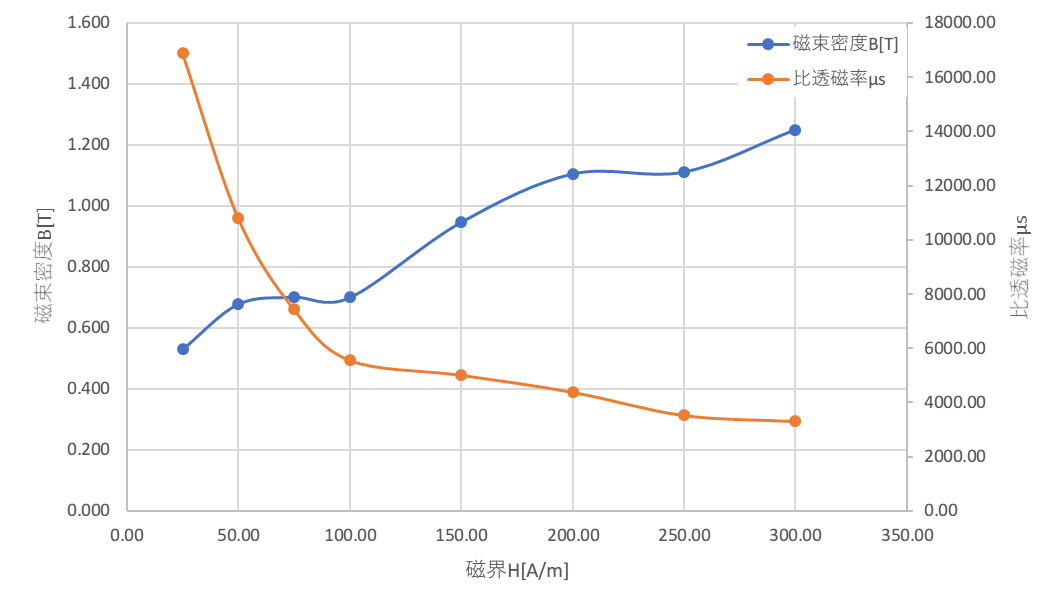
\includegraphics[height=10cm]{./fig/3.png}
  \caption{磁界に対する磁束密度と比透磁率の関係}
\end{figure}

\begin{table}[htbp]
  \centering
  \caption{電気鉄板の鉄損測定(f=50Hz)}
  \scalebox{0.61} {
    \begin{tabular}{@{}rrrr@{}}
  \toprule
  \multicolumn{1}{c}{負荷抵抗} & \multicolumn{1}{c}{発電電圧{[}V{]}} & \multicolumn{1}{c}{発電電流{[}mA{]}} & \multicolumn{1}{c}{電力{[}mW{]}} \\ \midrule
  0  & 2.3 & 8  & 18.4\\
  5  & 2.2 & 9  & 19.8\\
  10 & 2.1 & 9  & 18.9\\
  15 & 2.0 & 8  & 16.0\\
  20 & 2.0 & 9  & 18.0\\
  25 & 1.9 & 9  & 17.1\\
  30 & 1.6 & 9  & 14.4\\
  35 & 1.5 & 9  & 13.5\\
  40 & 1.4 & 8  & 11.2\\
  45 & 1.3 & 8  & 10.4\\
  50 & 1.2 & 8  & 9.6 \\
  55 & 1.0 & 9  & 9.0 \\
  60 & 0.9 & 9  & 8.1 \\
  65 & 0.8 & 9  & 7.2 \\
  70 & 0.7 & 9  & 6.3 \\
  75 & 0.6 & 9  & 5.4 \\
  80 & 0.5 & 9  & 4.5 \\
  85 & 0.3 & 9  & 2.7 \\
  90 & 0.2 & 9  & 1.8 \\
  95 & 0.1 & 9  & 0.9 \\
  100 & 0.1 & 1 & 0.1 \\ \bottomrule
\end{tabular}
  }
\end{table}

\begin{table}[htbp]
  \centering
  \caption{電気鉄板の鉄損測定(f=60Hz)}
  \scalebox{0.61} {
    \begin{tabular}{@{}rrrr@{}}
  \toprule
  \multicolumn{1}{c}{負荷抵抗} & \multicolumn{1}{c}{発電電圧{[}V{]}} & \multicolumn{1}{c}{発電電流{[}mA{]}} & \multicolumn{1}{c}{電力{[}mW{]}} \\ \midrule
  0   & 12.3 & 57 & 701.1\\
  5   & 12.0 & 58 & 696.0\\
  10  & 11.4 & 58 & 661.2\\
  15  & 10.7 & 59 & 631.3\\
  20  & 10.7 & 59 & 631.3\\
  25  & 9.8  & 60 & 588.0\\
  30  & 9.8  & 60 & 588.0\\
  35  & 8.3  & 61 & 506.3\\
  40  & 7.7  & 61 & 469.7\\
  45  & 7.1  & 62 & 440.2\\
  50  & 6.3  & 62 & 390.6\\
  55  & 5.6  & 62 & 347.2\\
  60  & 5.0  & 63 & 315.0\\
  65  & 4.4  & 63 & 277.2\\
  70  & 3.7  & 64 & 236.8\\
  75  & 3.0  & 64 & 192.0\\
  80  & 2.3  & 64 & 147.2\\
  85  & 1.6  & 65 & 104.0\\
  90  & 1.2  & 64 & 76.8 \\
  95  & 0.4  & 64 & 25.6 \\
  100 & 0.1  & 64 & 6.4  \\ \bottomrule
\end{tabular}
  }
\end{table}

\begin{figure}[H]
  \centering
  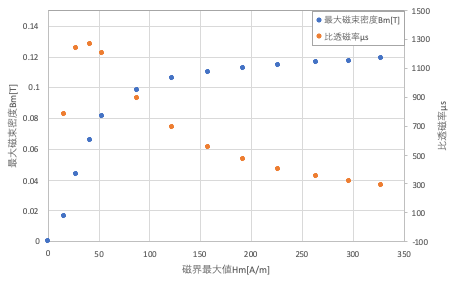
\includegraphics[height=10cm]{./fig/4.png}
  \caption{磁界に対する最大磁束密度と比透磁率の関係(f=50Hz)}
\end{figure}

\begin{figure}[H]
  \centering
  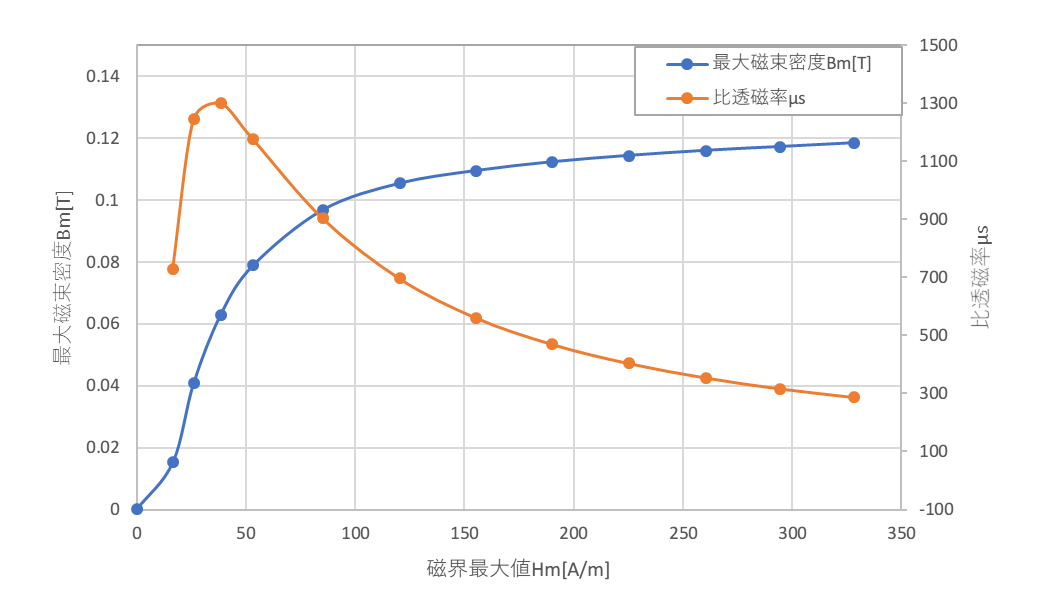
\includegraphics[height=10cm]{./fig/5.png}
  \caption{磁界に対する最大磁束密度と比透磁率の関係(f=60Hz)}
\end{figure}

\begin{figure}[H]
  \centering
  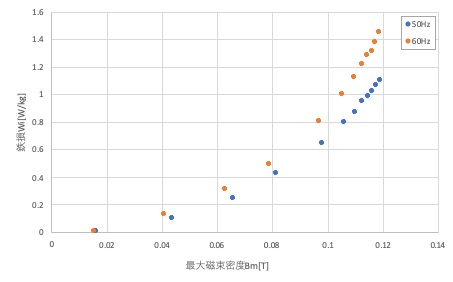
\includegraphics[height=10cm]{./fig/6.png}
  \caption{最大磁束密度に対する鉄損の関係}
\end{figure}

\newpage
\section{考察}
 磁束計による電気機器用鉄板の B-H 曲線の測定では,

 図4と図5を比較すると,グラフの概形,はほぼ一致していた.このことから,磁界に対する磁束密度,及び磁界に対する比透磁率は周波数に依存しないと考えられる.


\newpage
\theendnotes

\end{document}
